\begin{frame}{more targetted stealing/extortion}
\end{frame}


{
    \setbeamertemplate{navigation symbols}{}
    \begin{frame}[plain]
        \begin{tikzpicture}[remember picture,overlay]
            \node[at=(current page.north),anchor=north] {
                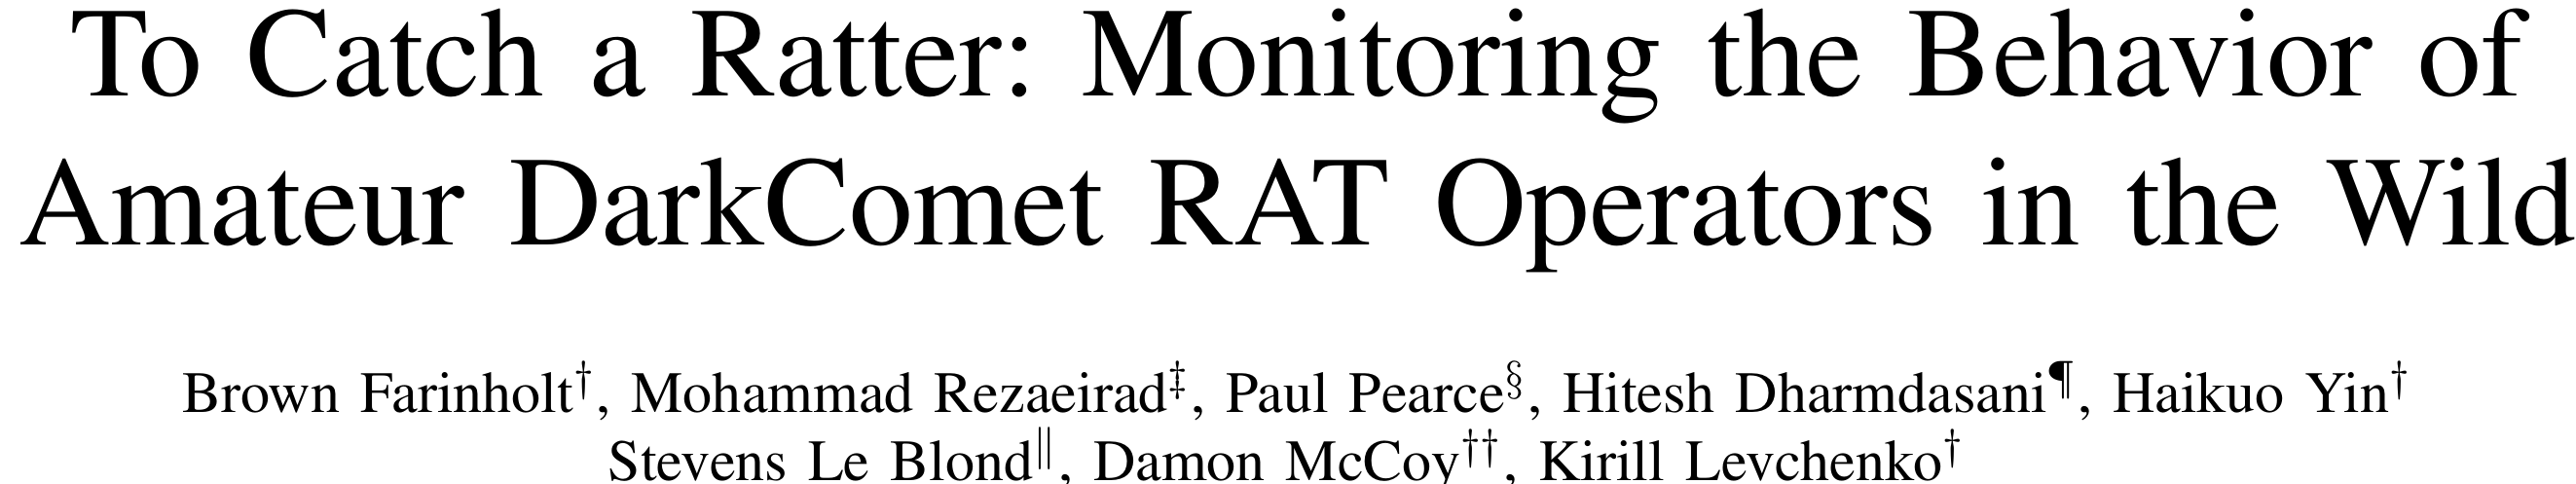
\includegraphics[width=0.8\paperwidth]{../intro/catch-ratter-title}
            };
            \node[at=(current page.south),anchor=south] {
                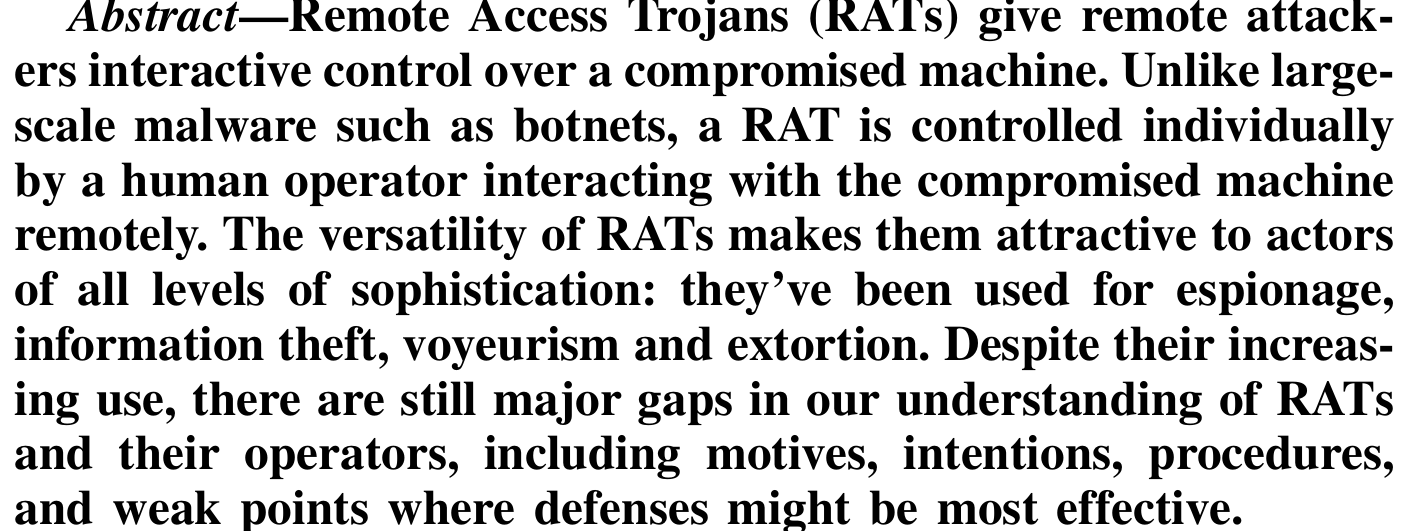
\includegraphics[height=0.5\paperheight]{../intro/catch-ratter-abs1}
            };
        \end{tikzpicture}
    \end{frame}
}

\begin{frame}{to catch ratter results}
    \begin{itemize}
    \item 2016/7 study
    \item 61\% attempt to access webcam; 26\% microphone
        \begin{itemize}
        \item (both not present in experimenter's `honeypot')
        \end{itemize}
    \item 31\% enable keylogger (passwords?)
    \item approx. 5\% harass legit user
    \item approx. 2\% try to phish legit user
    \end{itemize}
\end{frame}

